\documentclass[12pt]{article}
\usepackage{graphicx}
\usepackage {color}
\usepackage{pdfpages}
\usepackage{float}
\usepackage{changebar}
\usepackage{enumitem,amssymb}
\renewcommand{\familydefault}{\sfdefault}
\usepackage[margin=1.2in]{geometry}
\usepackage{graphicx}
\usepackage{wrapfig}
\usepackage[super]{cite}
\usepackage{subcaption}
\usepackage[table]{xcolor}
\usepackage{amsmath}
\usepackage[sort, numbers]{natbib}
\usepackage{multirow}
\usepackage{tabularx}
\usepackage{siunitx}
\usepackage{matlab-prettifier}
%%%%%%%%%%%%Defining the margins %%%%%%%%%%%%%%%%%%%%%
\textheight 9.in
\textwidth 6.5in
\topmargin -.5in
\oddsidemargin 0in
\setlength{\parskip}{\smallskipamount}

%%%%%%%%%%%%%%Specific Commands %%%%%%%%%%%%%%%%%%
\newcommand{\eg}{{\em e.g.,}}
\newcommand{\ie}{{\em i.e.,}}
\newcommand{\etc}{{\em etc.,}}
\newcommand{\etal}{{\em et al.}}
\newcommand{\degrees}{{$^{\circ}$}}
\newcommand{\fig}[1]{\textbf{Figure #1}}

%%%%%%%%%%%%%%%%%%%%%%%%%%%% Setting to control figure placement
% These determine the rules used to place floating objects like figures 
% They are only guides, but read the manual to see the effect of each.
\renewcommand{\topfraction}{.9}
\renewcommand{\bottomfraction}{.9}
\renewcommand{\textfraction}{.1}
\renewcommand{\familydefault}{\sfdefault} %setting the san serif font

%%%%%%%%%%%%%%%%%%%%%%%% Line spacing
% Use the following command for ``double'' spacing
%\setlength{\baselineskip}{1.2\baselineskip}
% and this one for an acceptable NIH spacing of 6lpi based on 11pt
%\setlength{\baselineskip}{.9\baselineskip}
% The baselineskip does not appear to work when we include a maketitle
% command in the main file.  Something there must set the line spacing
% If we use this next command, then things seem to work.
\renewcommand{\baselinestretch}{.9}

\setcounter{secnumdepth}{0} %make no numbers but have a table of contents


\begin{document}

\title{HW 2: Medical Imaging Systems}
\author{Jake Bergquist, u6010393 }
\maketitle

\section{Q1}\
a)Goal: Derive the following relationship\\
$M_0 = \frac{N\gamma^2h^2}{16\pi^2kT}B_0$\\
To begin with I will lay out some of the foundational assumptions and relationships based on class lecture.\\

\begin{equation}
\hbar = \frac{h}{2\pi}
\label{eq1}
\end{equation}
\begin{equation}
N_+ + N_- = N
\label{eq2}
\end{equation}
\begin{equation}
N_- \approxeq \frac{N}{2}
\label{eq3}
\end{equation}
\begin{equation}
\mu = \gamma \hbar I
\label{eq4}
\end{equation}
\begin{equation}
E = -\mu B_0 = -\gamma \hbar I B_0
\label{eq5}
\end{equation}
\begin{equation}
\frac{N_+}{N_-} = e^{\frac{-\Delta E}{kT}}
\label{eq6}
\end{equation}
\begin{equation}
M_0 = \frac{(N_+ - N_-)\gamma \hbar}{2}
\label{eqKey}
\end{equation}
The first step I will take is to break $\Delta E$ into $E_+ - E_-$ by definition. By then substituting the definitions for $E$ from Eq~\ref{eq5} into Eq~\ref{eq6} we get Eq~\ref{eq7} below (after distributing the negative and using $I = 1/2$ for $E_+$ and $I = -1/2$ for $E_-$).

\begin{equation}
\frac{N_+}{N_-} = e^{\frac{-(E_+-E_-)}{kT}} = e^{\frac{\gamma \hbar \frac{1}{2} B_0 + \gamma \hbar \frac{1}{2} B_0}{kT}}
\label{eq7}
\end{equation}

The term in the numerator of the exponential combines to give $\gamma \hbar B_0$. When $e^x$ and $x$ is small in magnitude $e^x \approxeq 1+ x$. Using this approximation we can reduce Eq~\ref{eq7} by converting the exponential as shown here and then miltpiling $N_-$ over. This yields Eq~\ref{eq8} below.
\begin{equation}
N_+ = N_- + \frac{N_- \gamma \hbar  B_0}{kT}
\label{eq8}
\end{equation}

By subtracting $N_-$ over and applying the approximation of Eq~\ref{eq3} we get Eq~\ref{eq9}

\begin{equation}
N_+ - N_- = \frac{N \gamma \hbar  B_0}{2kT}
\label{eq9}
\end{equation}

By substituting this quantity into Eq~\ref{eqKey} and substituting out $\hbar$ according to Eq~\ref{eq1} we get our final result.

b) at the given dimensions, each voxel would have dimensions of $24/192 cmx 24/192 cmx 1.0mm = 1.25 mm x 1.25 mm x 1.0 mm$ giving us a volume of $1.6 mm^3$ per voxel. $85\%$ of this volume is occupied by water in our tumor. Water has a density of $~1 g/cm^3 = 0.001 g/mm^3$ giving us $1.6 mm^3 * 85\% * 0.001g/mm^3 = 0.0014 g$ of water. At an atomic mass of 18 g/mole, at at a mass of 0.0014 g this gives us $\frac{0.0014 g}{18 g/mole} = 7.8*10^{-5}mole$ of water molecules. At 2 hydrogen per water molecule this gives us a total of $1.6*10^{-4} mole$ of hydrogen atoms or $9.6 * 10^{19} $ hydrogen nucli in water molecules. Assuming a body temperature of 310.15 K (37 Celsius), knowing that $\gamma/2*\pi = 42.58 MHz/T$ for hydrogen nuclei, with a 3 T magnet:\\ $M_0 = \frac{N\gamma^2h^2}{16\pi^2kT}B_0 =\frac{Nh^2}{4kT}\frac{\gamma^2}{4\pi^2}B_0 = \frac{9.6 * 10^{19}* (6.6*10^{-34} J*s)^2}{4*(1.4*10^{-23} J/K)*310.15 K}(42.58 MHz/T)^2*3T$\\
$\frac{9.6 * 10^{19}* (6.6*10^{-34} J*s)^2}{4*(1.4*10^{-23} J/K)*310.15 K}(4.258 * 10^7 Hz/T)^2*3T = 9.4*10^{-12}J/T$\\

Addressing the unit conversions:\\
$\frac{ (J*s)^2}{J/K*K}\frac{Hz^2*T}{T^2} = J*s^2\frac{1}{T*s^2} = J/T$


\section{Q2}
\subsection{a}
To begin with, from lecture we know EQ~\ref{eq10}

\begin{equation}
M_z(t) = M_{zinitial}  e^{-\frac{t}{T_1}} + m_0(1-e^{-\frac{t}{T_1}})
\label{eq10}
\end{equation}

This can be reformulated in terms of the steady state $M_Z$ which will occur at TR time. Once at steady state the $M_{zinitial} = M_z^{ss}cos(\alpha)$ because at this steady state after each excitation it is the steadtystate magnitude that will determine what the initial Mz value will be.Thus we get Eq~\ref{eq11}. By solving for $M_z^{ss}$ we get Eq~\ref{eq12} which is our desired steady state longitudinal magnetization.

\begin{equation}
M_z^{ss} = M_z(TR) = M_z^{ss}  e^{-\frac{TR}{T_1}} + m_0(1-e^{-\frac{TR}{T_1}})
\label{eq11}
\end{equation}

\begin{equation}
M_z^{ss} =\frac{m_0(1-e^{-\frac{TR}{T_1}})}{1- cos(\alpha)e^{-\frac{TR}{T_1}}}
\label{eq12}
\end{equation}

\subsection{b}
The above describes the magnitude of the $M_z^{ss}$ but the observed/measured magnitude must be in the xy plane in order to be measured by the receiving coil. Thus the observed steady state longitudinal magnitization is given by Eq~\ref{eq13}.

\begin{equation}
M_{zobserved}^{ss} =M_{z}^{ss}sin(\alpha) = \frac{sin(\alpha)m_0(1-e^{-\frac{TR}{T_1}})}{1- cos(\alpha)e^{-\frac{TR}{T_1}}}
\label{eq13}
\end{equation}

In order to find the flip angle ($\alpha$) that gives the greatest observed signal we must differentiate Eq~\ref{eq13} with respect to $\alpha$, set this equal to zero and solve for the alpha that maximizes intensity. We must then check that this alpha is indeed a maxima. In order to make this process simpler, terms in Eq~\ref{eq13} that are constant and do not change with respect to $\alpha$ will be lumped into constant terms. such that $C_1 = m_0(1-e^{-\frac{TR}{T_1}})$, and $C_2 = e^{-\frac{TR}{T_1}}$. Additionally the denominator will be brought up as a term with a negative exponent so that the product rule (rather than the quotent rule) can be used (by preference). The resulting simplification is shown in Eq~\ref{eq14}.

\begin{equation}
M_{zobserved}^{ss} = C_1sin(\alpha)(1- C_2cos(\alpha))^{-1}
\label{eq14}
\end{equation}

Using the product rule and the chain rule this can be differentiated into the form seen in Eq~\ref{eq15} and simplified to Eq~\ref{eq16} by setting the derivative equal to zero and rearranging.

\begin{equation}
\frac{d}{d\alpha} = (1- C_2cos(\alpha))^{-1} C_1cos(\alpha) + C_1sin(\alpha)(-(1- C_2cos(\alpha))^{-2})C_2sin(\alpha)
\label{eq15}
\end{equation}
\begin{equation}
\frac{C_1cos(\alpha)}{1-C_2cos{\alpha}} = \frac{C_1C_2sin^2(\alpha)}{(1-C_2cos{\alpha})^2}
\label{eq16}
\end{equation}

Eq~\ref{eq16} can be used to solve for the $\alpha$ that sets the derivative to 0 (either a maxima or minima) by canceling like terms, and applying a trig identity ($sin^2 = 1-cos^2$). These steps are carried out in Eq~\ref{eq17}~-~\ref{eq21}.

\begin{equation}
cos(\alpha) = \frac{C_2sin^2(\alpha)}{1-C_2cos{\alpha}}
\label{eq17}
\end{equation}

\begin{equation}
cos(\alpha) - c_2cos^2(\alpha) = C_2(1-cos^2(\alpha))
\label{eq18}
\end{equation}

\begin{equation}
cos(\alpha) - c_2cos^2(\alpha) = C_2-C_2cos^2(\alpha))
\label{eq19}
\end{equation}

\begin{equation}
cos(\alpha) = C_2
\label{eq20}
\end{equation}

\begin{equation}
\alpha = arccos(C_2) = arccos(e^{-\frac{TR}{T_1}})
\label{eq21}
\end{equation}

In order to confirm that this is the maxima I chose to plot the values of the observed intensities at a range of angles and observe where the maxima occured as compared to what would be na\"ive guess of the angle that maximized signals. The code used to do so is shown below and the resulting curve is shown in Figure~\ref{Fig:alphas}. As can be seen the maxima occures as calculated at an angle of $arccos(C_2)$. By comparison I might have expected the value to come at around $\frac{\pi}{2}$ as this would result in the entirety of Mz being excited into the xy plane, this is not the case. This is likely because if 90 degrees was chosen for the flip angle then it steady state longitudinal magnitude would be smaller, leading to a smaller signal when it is flipped into the xy plane.


\begin{lstlisting}[style=Matlab-editor]
%%
%Q2
C2 = exp(-5/5);
C1 = 5*(1-C2);
alps = [0:.01:3.14];
Mzs = C1*sin(alps)./(1-C2*cos(alps));
figure(1);clf();plot(alps,Mzs,'linewidth',2);hold on;
scatter(pi/2,C1*sin(pi/2)/(1-C2*cos(pi/2)),'ro');
scatter(acos(C2),C1*sin(acos(C2))/(1-C2*cos(acos(C2))),'bo');
ylabel('Observed M_z');
xlabel('Aplha Values');
set(gca,'fontsize',18)


\end{lstlisting}

\begin{figure}[H]
	\centering
	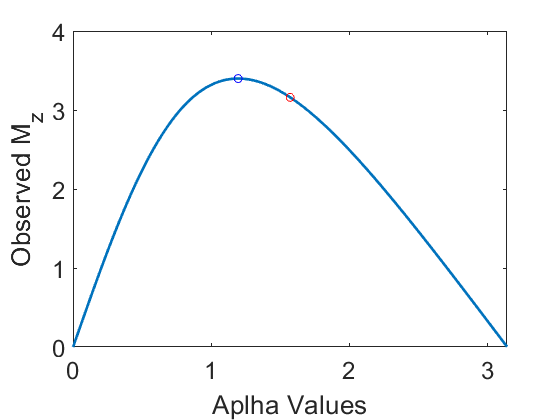
\includegraphics[width=\textwidth]{alphavsmz.png}
	\caption{Alpha values vs the observed $M_z$ for each at steady state. The red circle indicates the intensity at $\alpha = pi/2$ and the blue circle indicates the intensity at $\alpha = C_2 = e^{-\frac{TR}{T_1}}$.}
	\label{Fig:alphas}
\end{figure}

%%%%%%%%%%%%%%%%%% Correct Bibliography Style

\section{Q3}
A simple method can be used to calculate the $T_1$ and $T_2$ using Eq~\ref{eq22}. $I_0$ seems like a troubling quantity but it can be eliminated by taking multiple measurements and using their ratio to cancel out common terms. By making three measurements both T values can be measured. The first measurement uses essentially a random TE and TR. These should be selected to be within normal ranges, and their values shoudl be reasonable but it is not imporant what specific values are chosen from a purely theoretical point of view. Tehcnical limitations and practicalities of measurement will likely inform their selection. What is important is what is done next. These first values are called $TE_1$ and $TR_1$ respectively. A second set of parameters must be selected that are different from  $TE_1$ and $TR_1$ which we call  $TE_2$ and $TR_2$ respectively. Again their selection will be based on practical concerns about the measurement system, the only important thing is that they be different from  $TE_1$ and $TR_1$. Three measurements of intensity will be taken using these values. One measurement using  $TE_1$ and $TR_1$, one using $TE_1$ and $TR_2$, and a final one using $TE_2$ and $TR_1$. Notice how in the second two measurements either TE or TR was changed from the first measurement but not both. These measurements produce intensity values of $I_1$, $I_2$, and $I_3$ respectively. By forming Ratios of either $\frac{I_1}{I_2}$ or $\frac{I_1}{I_3}$ we create scenarios where only TR or TE vary respectively. In the case of ratio 1 ($\frac{I_1}{I_2}$), all terms cancel out from Eq~\ref{eq22} except for those that involve TR. Thus the ratio 1 is dictated by $T_1$ and thus the ratio equation can be rearreanged to solve for $T_1$. The same principle is applied for Ratio 2 ($\frac{I_1}{I_3}$) to get a scenario that depends only on $T_2$. In this way three measurements can be used to calculate both recovery times. This scenario of course assumes minimal/no noise. Real noise would necessitate multiple recordings in order to average the noise and minimize its impact on the relaxation time calculations.
\begin{equation}
I = I_0(1-e^{-\frac{TR}{T_1}})e^{-\frac{TE}{T_2}}
\label{eq22}
\end{equation}

\section{Q4}
\subsection{a: }
Eq~\ref{eq22} can be used to calculate the "T2-weighted" spin echo intensity. By fixing TR the second term (involving T1) becomes constant and can be combined with $I_0$. This term I call $I^* = I_0(1-e^{\frac{TR}{T_1}})$. This gives us Eq~\ref{eq23}.
\begin{equation}
I = I^*e^{-\frac{TE}{T_2}}
\label{eq23}
\end{equation}

Taking the natural logarithm of both sides of this function and separating out $I^*$ and T2 dependent parts using one of the logarithm rules we get Eq~\ref{eq24} which simplifies to Eq~\ref{eq25}

\begin{equation}
ln(I) = ln(I^*) + ln(e^{-\frac{TE}{T_2}})
\label{eq24}
\end{equation}
\begin{equation}
ln(I) = -\frac{1}{T_2}TE + ln(I^*) 
\label{eq25}
\end{equation}

Eq~\ref{eq25} shows a familiar $y = mx + b$ linear form where the slope is given by $ -\frac{1}{T_2}$ and the y intercept is given by $ln(I^*)$. The $ln(I)$ term is the dependent variable while the TE is the independent variable. The $ -\frac{1}{T_2}$ and $I^*$ terms are unknown that could be solved for by fitting measured data to this equation form.

\subsection{b}
The code below was used to calculate the T2 and $I^*$ for both the background and the tumor data. For the tumor T2 was found to be 84.1 ms and $I^*$ was $1.4*10^3$. For the background/surrounding tissue the T2 was 79.0 and the $I^*$ was 187.9. We can evaluate the fits by looking at the measured and fit curves in both the linearized and non-linear views. For the tumor data, Figure~\ref{fig:tumor} shows the fit and measured curves. As can be seen the linearized fit aggrees well with the data. Roughly 50\% of the data appears to be above and 50\% below the fit line and the distance between fit and measured is very small. When observing the non-linear view (Figure~\ref{fig:t_nonlin}) we see again that the fit seems to match well, almost appearing as a spline interpolation between the measured points as opposed to the red linear interpolation. The fit results for the background/surrounding tissue are worse. Figure~\ref{fig:bckgrnd} shows these fitting results. In the linearized view, while still roughly 50\% of the measured points lie on either side of the fit line the distance to the fit line is much higher. The linearized data itself is very spread out, implying a higher amount of noise in this area. This could be due to the lower amplitude of the signal and therefor lower SNR. The resulting fit on the non-linear view is very poor, and it seems that fitting this data without linearizing may have actually resulted in a better fit.

\begin{lstlisting}[style=Matlab-editor]
%Q4

TE = [10 20 30 50 100 250];
tumor = [1213.4 1099.3 994.7 783.2 447.6 70.9];
background = [448.1 306.7 239.1 119.0 1.1 30.4];

%Fit the tumor unknowns
coeffs_tumor = polyfit(TE,log(tumor),1);
T2_tumor = -1/coeffs_tumor(1);
IndependedntIntensity_Tumor = exp(coeffs_tumor(2));
%visualize both linearlize dand original
figure(1);clf();hold on;plot(TE,tumor,'r','linewidth',2);
plot([10:1:250],IndependedntIntensity_Tumor*exp(-[10:1:250]/T2_tumor),'b','linewidth',2)
xlabel('TE (msec)');ylabel('intensity');set(gca,'fontsize',18);
figure(2);clf();hold on;plot(TE,log(tumor),'r','linewidth',2);
plot([10:1:250],coeffs_tumor(1).*[10:1:250]+coeffs_tumor(2),'b','linewidth',2);
xlabel('TE (msec)');ylabel('intensity');set(gca,'fontsize',18);

%Fit for background
coeffs_background = polyfit(TE,log(background),1);

T2_background = -1/coeffs_background(1);
IndependedntIntensity_background = exp(coeffs_background(2));
%visualize both linearlize dand original
figure(3);clf();hold on;plot(TE,background,'r','linewidth',2);
plot([10:1:250],IndependedntIntensity_background*exp(-[10:1:250]/T2_background),'b','linewidth',2)
xlabel('TE (msec)');ylabel('intensity');set(gca,'fontsize',18);
figure(4);clf();hold on;plot(TE,log(background),'r','linewidth',2);
plot([10:1:250],coeffs_background(1).*[10:1:250]+coeffs_background(2),'b','linewidth',2);
xlabel('TE (msec)');ylabel('intensity');set(gca,'fontsize',18);


\end{lstlisting}


\begin{figure}[H]
	\begin{subfigure}{.5\textwidth}
		\centering
		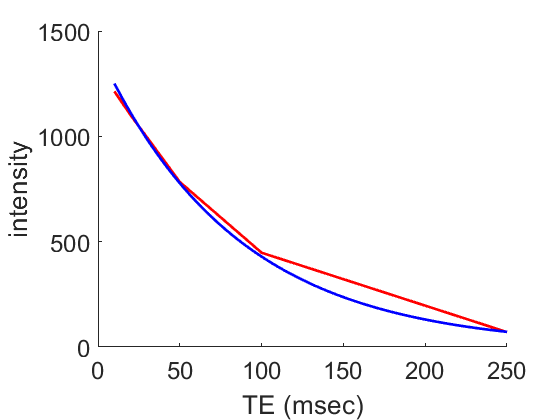
\includegraphics[width=.95\linewidth]{tumor_nonlin.png}
		\caption{}
		\label{fig:t_nonlin}
	\end{subfigure}%
	\begin{subfigure}{.5\textwidth}
		\centering
		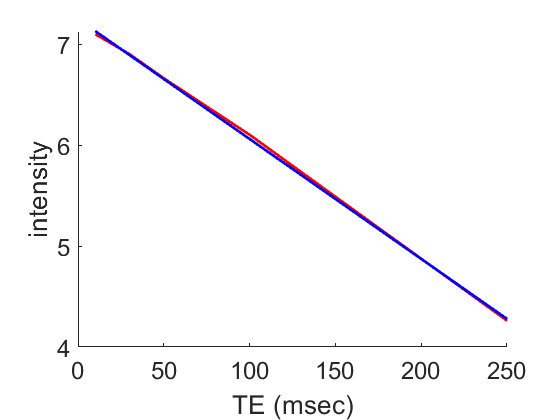
\includegraphics[width=.95\linewidth]{tumor_lin.png}
		\caption{}
		\label{fig:t_lin}
	\end{subfigure}
	\caption{Results of fitting the tumor data (red) and plotting using the fit parameters (blue) and Eq~\ref{eq23} (a) or \ref{eq25} (b). a shows the non-linearized measured data and fitline, while b shows the linearized data and fitline.}
	\label{fig:tumor}
\end{figure}


\begin{figure}[H]
	\begin{subfigure}{.5\textwidth}
		\centering
		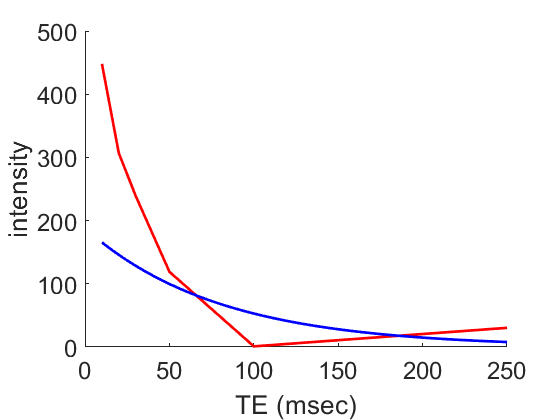
\includegraphics[width=.95\linewidth]{bck_nonlin.png}
		\caption{}
		\label{fig:b_nonlin}
	\end{subfigure}%
	\begin{subfigure}{.5\textwidth}
		\centering
		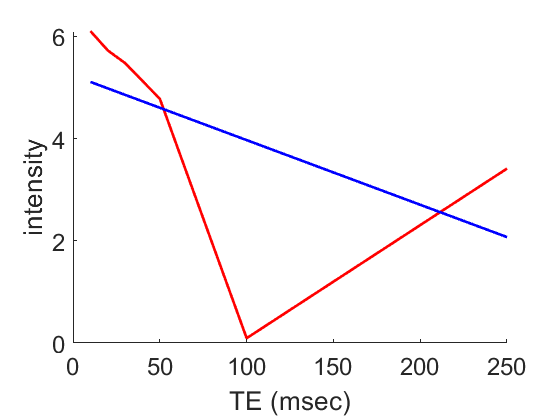
\includegraphics[width=.95\linewidth]{bck_lin.png}
		\caption{}
		\label{fig:b_lin}
	\end{subfigure}
	\caption{Results of fitting the background data (red) and plotting using the fit parameters (blue) and Eq~\ref{eq23} (a) or \ref{eq25} (b). a shows the non-linearized measured data and fitline, while b shows the linearized data and fitline.}
	\label{fig:bckgrnd}
\end{figure}

\subsection{c}
To maximize contrast we must maximize Eq~\ref{eq26} with respect to TE where $T_{2t}$ is the T2 for the tumor, $T_{2b}$ is the T2 for the background, $I^*_T$ is the $I^*$ for the tumor, and $I^*_b$ is the $I^*$ for the background.
\begin{equation}
I_{tumor}-I_{background} = I^*_Te^{-\frac{TE}{T_{2t}}}-I^*_be^{-\frac{TE}{T_{2b}}} 
\label{eq26}
\end{equation}
Taking the derivative and setting it equal to zero then solving for TE gives the maximizing TE. This is seen in EQ~\ref{eq29}~-~\ref{eq34}.
\begin{equation}
\frac{d}{dTE}I_{tumor}-I_{background} = -\frac{I^*_T}{T_{2t}}e^{-\frac{TE}{T_{2t}}}+\frac{I^*_b}{T_{2b}}e^{-\frac{TE}{T_{2b}}} => 0
\label{eq29}
\end{equation}
\begin{equation}
\frac{I^*_b}{T_{2b}}e^{-\frac{TE}{T_{2b}}}=\frac{I^*_T}{T_{2t}}e^{-\frac{TE}{T_{2t}}}
\label{eq30}
\end{equation}
\begin{equation}
e^{-\frac{TE}{T_{2b}}}e^{\frac{TE}{T_{2t}}}=\frac{I^*_TT_{2b}}{I^*_bT_{2t}}
\label{eq31}
\end{equation}
\begin{equation}
ln(e^{TE(\frac{1}{T_{2t}}-\frac{1}{T_{2b}})})=\ln(\frac{I^*_TT_{2b}}{I^*_bT_{2t}})
\label{eq32}
\end{equation}
\begin{equation}
TE(\frac{1}{T_{2t}}-\frac{1}{T_{2b}})=ln(\frac{I^*_TT_{2b}}{I^*_bT_{2t}})
\label{eq33}
\end{equation}
\begin{equation}
TE_{max}=\frac{ln(\frac{I^*_TT_{2b}}{I^*_bT_{2t}})}{\frac{1}{T_{2t}}-\frac{1}{T_{2b}}} = \frac{ln(\frac{1400*79.0}{187.9*84.1})}{\frac{1}{84.1}-\frac{1}{79.0}} = -2.5*10^3
\label{eq34}
\end{equation}

The TE value we get is negative as seen in EQ~\ref{eq34}, however we can take the absolute value of this TE to get out desired TE, seeing as pixel contrast is an absolute value measurement of the difference between the intensities. This negation could also be corrected by flipping the order of the intensities int he original contrast definition. Thus $TE_{max} = 2.5*10^3 msec$.

\section{Q5}
\subsection{a}
Generically we have Eq~\ref{eq10}. In our case of a 180 degree pulse $M_{initial} = m_0cos(\alpha) = -M_0$. Substituting this into Eq~\ref{eq10} and distributing $M_0$ in the second term gives the relationship and simplification shown in Eq~\ref{eq28} which is the longitudinal magnetization as a function of $T_1$, $TI$, and $M_0$ where $t = TI$. Because these are magnitudes we do not need to worry about projecting the value into the xy plane using a second flip. 

\begin{equation}
M_z(t) = -M_0  e^{-\frac{t}{T_1}} + m_0-M_0e^{-\frac{t}{T_1}}) = M_0(1-2e^{-\frac{t}{T_1}})
\label{eq28}
\end{equation}

\subsection{b}
Before we can get to curve fitting we must first address a problem. Because the intensities measured are absolute value, and we have done a 180 degree pulse there is an artifact in the signal due to this absolute value measurement. This makes the curves look more like check marks. This can be seen in the table as the values first are decreasing then increasing as TI increases. To fix this the first three values in both rows of the table must be negated. Otherwise fitting will fail.
The code below was used for this fitting using fminsearch and an objective function that produced the squared difference between the measurements and Eq~\ref{eq28}, optimizing over $M_0$ and $T_1$. 500 and 500 were selected as initial guesses in both cases because it was found that using a small number such as 1 or 0 resulted in a poor fit. $M_0$ was found to be 972 J/s and 359 J/s for tissue 1 and 2 respectively. the $T_1$ was found to be 609 msec 409 msec for tissue 1 and 2 respectively. The resulting fits (Figure~\ref{fig:tissuefits}) show good visual agreement.
\begin{lstlisting}[style=Matlab-editor]
%Q5
TI = [50 100 200 400 800 1600];
tissue1 = [-889 -684 -461 99.4 385 780];
tissue2 = [-261 -217 -108 118 254 339];

objFunc_tiss1 = @(param) LongMagIntensity(TI,tissue1,param);
optParams_tiss1 = fminsearch(objFunc_tiss1,[500,500]);
figure(1);clf();hold on;
plot(TI,tissue1,'r','linewidth',2);
plot([50:1600],optParams_tiss1(1).*(1-2*exp(-[50:1600]/optParams_tiss1(2))),'b','linewidth',2);
xlabel('TI (msec)');ylabel('intensity');set(gca,'fontsize',18);

objFunc_tiss2 = @(param) LongMagIntensity(TI,tissue2,param);
optParams_tiss2 = fminsearch(objFunc_tiss2,[500,500]);
figure(2);clf();hold on;
plot(TI,tissue2,'r','linewidth',2);
plot([50:1600],optParams_tiss2(1).*(1-2*exp(-[50:1600]/optParams_tiss2(2))),'b','linewidth',2);
xlabel('TI (msec)');ylabel('intensity');set(gca,'fontsize',18);

function cost = LongMagIntensity(TI,m,param)
M0 = param(1);
T1 = param(2);
cost = sum((m - M0 * (1 - 2*exp(-TI/T1))).^2);

end
\end{lstlisting}

\begin{figure}[H]
	\begin{subfigure}{.5\textwidth}
		\centering
		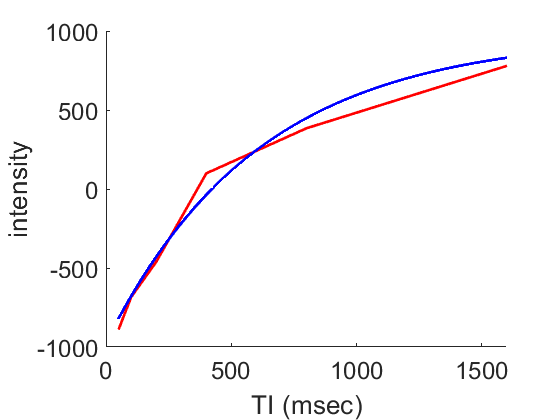
\includegraphics[width=.95\linewidth]{tissue1_fit.png}
		\caption{}
		\label{fig:t1fit}
	\end{subfigure}%
	\begin{subfigure}{.5\textwidth}
		\centering
		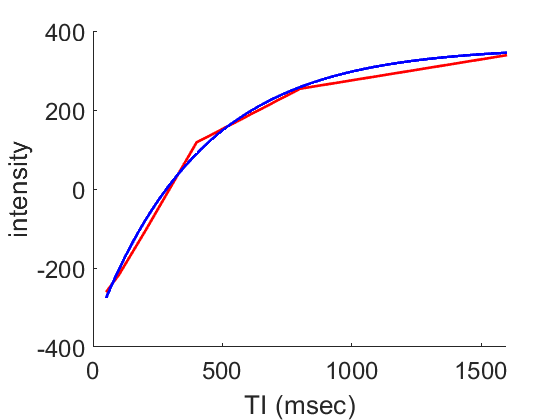
\includegraphics[width=.95\linewidth]{tissue2_fit.png}
		\caption{}
		\label{fig:t2fit}
	\end{subfigure}
	\caption{Results of fitting the data for each tissue (red) and plotting using the fit parameters (blue) and Eq~\ref{eq28}. (a) shows the data and fit for tissue 1, while (b) shows the data and fit for tissue 2.}
	\label{fig:tissuefits}
\end{figure}

\section{c}
Like in problem 4 we need to take the derivative of our equation of inters (EQ~\ref{eq28}) in the formulation of contrast between two measurements with respect to TI where t=TI. The contrast eqation is shown in EQ~\ref{eq35}and the resulting derivative and solution for the maximizing TI are shown in EQ~\ref{eq36}~-~\ref{eq39} where $T_{1a}$ is the $T_1$ of tissue 1, $T_{1b}$ is the $T_1$ of tissue 2, $M_{0a}$ is the $M_0$ of tissue 1, and $M_{0b}$ is the $M_0$ of tissue 2.

\begin{equation}
M_{za}-M_{zb} = M_{0a}(1-2e^{-\frac{TI}{T_{1a}}})-M_{0b}(1-2e^{-\frac{TI}{T_{1b}}})
\label{eq35}
\end{equation}
\begin{equation}
\frac{d}{dTI}(M_{za}-M_{zb})= -\frac{-2M_{0a}}{T_{1a}}e^{-\frac{TI}{T_{1a}}}+\frac{-2M_{0b}}{T_{1b}}e^{-\frac{TI}{T_{1b}}} => 0
\label{eq36}
\end{equation}

\begin{equation}
\frac{2M_{0b}}{T_{1b}}e^{-\frac{TI}{T_{1b}}}=\frac{2M_{0a}}{T_{1a}}e^{-\frac{TI}{T_{1a}}}
\label{eq37}
\end{equation}

\begin{equation}
e^{TI(\frac{1}{T_{1b}}-\frac{1}{T_{1a}})}= \frac{2M_{0b}T_{1a}}{2M_{0a}T_{1b}}
\label{eq38}
\end{equation}
\begin{equation}
TI_{maximizer}= \frac{ln(\frac{2M_{0b}T_{1a}}{2M_{0a}T_{1b}})}{\frac{1}{T_{1b}}-\frac{1}{T_{1a}}} = \frac{ln(\frac{359*609}{972*409})}{\frac{1}{409}-\frac{1}{609}} = -744msec
\label{eq39}
\end{equation}

Again like problem 4 the result is negative but can be taken at absolute value for the reasons explained in problem 4 part c. Thus the TI that maximizes the contrast for these two tissue for the LONGITUDINAL MAGNETIZATION is 744 msec.
\section{EC}
For any given sample the bulk magnetization of the sample is given by $\sum_{i = 1}^{N}\mu _i$ where $N$ is the number of spins in the sample and each $\mu$ is the individual magnetic vectors defined by Eq~\ref{eq4}. This is in the absence of a $B_0$ magnetic field. In a $B_0$ these vectors will align either with or against $B_0$ with energy described by EQ~\ref{eq5}. So far this is looking a lot like problem 1, we need a way to incorporate the individual spin states of these particles into the bulk magnetization shown in problem 1. I am not sure how to address this at the moment but I did find a resource online that described $|\mu| = \gamma \hbar \sqrt{I(I+1)}$ (http://mri.beckman.illinois.edu/interactive/topics/contents/basic\_concepts/index.shtml) where I is the spin quantum number referred to in this problem. I think that substituting this definition for $\mu$ and going through the derivation presented in problem 1 would be on the right track. I however am having trouble reconciling this definition with the ones we have used so far. 

\end{document}



\begin{figure}[H]
	\centering
	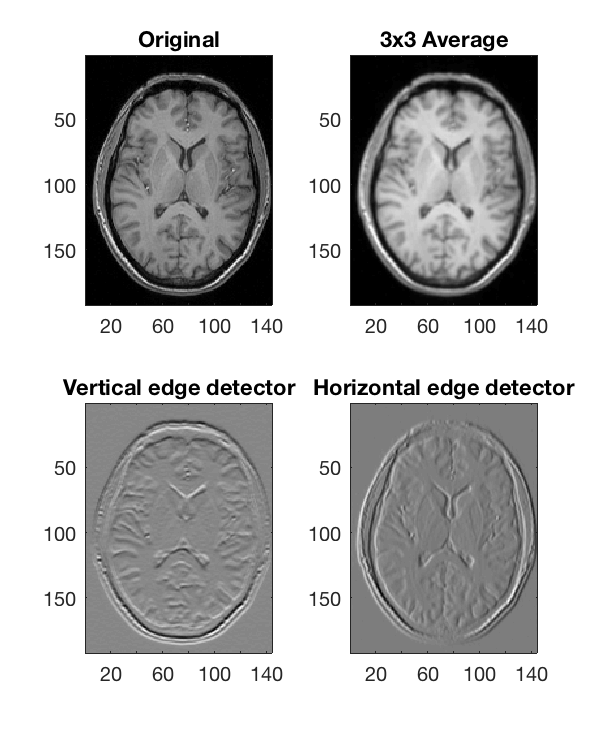
\includegraphics[width=\textwidth]{Figures/convs.png}
	\caption{}
	\label{Fig:conv}
\end{figure}






